\documentclass[11pt]{amsart}
\usepackage{amsmath,amssymb,amsthm}
\usepackage{booktabs}
\usepackage{tikz}
\usepackage[colorlinks=true,linkcolor=blue,citecolor=blue,urlcolor=blue]{hyperref}

\newtheorem{theorem}{Theorem}[section]
\newtheorem{proposition}[theorem]{Proposition}
\newtheorem{lemma}[theorem]{Lemma}
\newtheorem{corollary}[theorem]{Corollary}
\theoremstyle{definition}
\newtheorem{definition}[theorem]{Definition}
\newtheorem{question}[theorem]{Question}
\theoremstyle{remark}
\newtheorem{remark}[theorem]{Remark}

\newcommand{\R}{\mathbb{R}}
\newcommand{\rad}{\operatorname{rad}}
\newcommand{\diam}{\operatorname{diam}}
\newcommand{\tr}{^{\mathsf{T}}}
\newcommand{\lean}[1]{\texttt{#1}}

\begin{document}

\title[Laplacian spectral radius and second adjacency eigenvalue]{The gap between the
Laplacian spectral radius and the second adjacency eigenvalue of a graph}

\author{Sulaymon Sadullo}

\date{November 2026}

\subjclass[2020]{05C50; 15A42; 68V20}
\keywords{adjacency eigenvalues, Laplacian spectral radius, Randi\'c index, automated
conjectures, formal proof, Lean}

\begin{abstract}
Let $G$ be a connected graph, $\lambda_2$ the second largest eigenvalue of its adjacency matrix
and $\mu_1$ the largest eigenvalue of its Laplacian. It is known that
$\lambda_2\le\mu_1-1$. Cazenave recently conjectured, on the basis of a large corpus of
machine-generated conjectures, that $\lambda_2\le\mu_1-2$. We show that this fails for a graph
on $11$ vertices, and for some graph on $n$ vertices for every $n\ge 11$. We then show that the
known bound cannot be improved at all: the inequality $\lambda_2\le\mu_1-c$ holds for every
connected graph if and only if $c\le 1$. The extremal graphs are two complete split graphs
joined through a vertex of small degree. These results are formalized in Lean~4 with Mathlib.
On the same graphs the Randi\'c index $R$ satisfies $R-\lambda_2\to 1$ while the radius and the
diameter stay bounded, which refutes eighteen further open conjectures of the corpus. We also
report numerical evidence against about a hundred more.
\end{abstract}

\maketitle

\section{Introduction}

Throughout, $G$ is a finite simple connected graph with $n\ge 2$ vertices. We write
$\lambda_1\ge\lambda_2\ge\dots\ge\lambda_n$ for the eigenvalues of its adjacency matrix $A$ and
$\mu_1\ge\mu_2\ge\dots\ge\mu_n=0$ for those of its Laplacian $L=D-A$, where $D$ is the diagonal
matrix of degrees. The maximum degree is $\Delta$.

Inequalities between graph invariants have been produced by computer for a long time; Graffiti
\cite{Fajtlowicz} and AutoGraphiX \cite{CaporossiHansen} are the best known systems. Duhamel and
Cazenave \cite{DuhamelCazenave} recently generated a corpus of $305{,}755$ conjectures, each an
inequality between spectral and metric invariants of connected graphs. In \cite{Cazenave},
Cazenave reports that an automated pipeline refuted $162{,}964$ of them and proved $117{,}390$,
and he singles out seven of the remaining ones. The second is the following.

\medskip
\noindent\textbf{Conjecture 2 of \cite{Cazenave}.}
\emph{For every connected graph, $\lambda_2\le\mu_1-2$.}
\medskip

The conjecture is supported by paths, for which $\mu_1-\lambda_2$ decreases to $2$, and by an
exhaustive test on all connected graphs with at most $9$ vertices \cite{Cazenave}. With $1$ in
place of $2$ the inequality is true and easy: every adjacency eigenvalue is at most $\Delta$,
and $\mu_1\ge\Delta+1$ by a theorem of Grone and Merris \cite{GroneMerris}, so
\begin{equation}\label{eq:known}
\lambda_2\le\lambda_1\le\Delta\le\mu_1-1 .
\end{equation}
The same bound follows from Theorem~1 of \cite{Cazenave}, which states that
$\mu_2\ge\lambda_2+1$. The conjecture asks for one more unit. We show that there is nothing more
to be had.

\begin{theorem}\label{thm:G11}
Let $G_{11}$ be the graph of Figure~\ref{fig:G11}: two copies of $K_4$ minus an edge, joined by a
path with three inner vertices. Then $\mu_1(G_{11})\le\frac{37}{8}$ and
$\lambda_2(G_{11})\ge\frac{293}{111}$. Consequently
\[
\lambda_2(G_{11})-\bigl(\mu_1(G_{11})-2\bigr)\ \ge\ \tfrac{13}{888}\ >\ 0 ,
\]
and Conjecture~2 of \cite{Cazenave} is false.
\end{theorem}

\begin{theorem}\label{thm:family}
For every $n\ge 11$ there is a connected graph $G$ on $n$ vertices with
$\lambda_2(G)>\mu_1(G)-2$.
\end{theorem}

\begin{theorem}\label{thm:sharp}
Let $c$ be a real number. The inequality $\lambda_2(G)\le\mu_1(G)-c$ holds for every connected
graph $G$ with at least two vertices if and only if $c\le 1$.
\end{theorem}

In other words $\inf_G\,(\mu_1-\lambda_2)=1$. The infimum is not attained, because
$\lambda_2<\lambda_1$ for a connected graph. Theorem~\ref{thm:sharp} also disposes of two weaker
conjectures of the corpus, $\lambda_2\le\mu_1-\sqrt2$ and $\lambda_2\le\mu_1-\sqrt[4]{2}$; the
first of these is printed in the table of selected conjectures of \cite{DuhamelCazenave}.

The graphs behind Theorem~\ref{thm:sharp} are easy to describe. A \emph{cluster} is a complete
split graph: a clique on $m$ vertices together with $s$ further vertices, each joined to the
whole clique and to nothing else. The graph $T(m,s)$ consists of two clusters and one extra
vertex joined to one non-clique vertex of each (Figure~\ref{fig:T}). We prove
\begin{equation}\label{eq:gapbound}
\mu_1\bigl(T(m,s)\bigr)-\lambda_2\bigl(T(m,s)\bigr)\ \le\ 1+\frac{3}{s}+\frac{s^2-s}{m+s}
\qquad(m\ge2,\ s\ge2),
\end{equation}
and the right-hand side tends to $1$ when $s\to\infty$ and $m=s^3$.

The design is forced by \eqref{eq:known}. For $\mu_1-\lambda_2$ to be close to $1$ one needs
$\lambda_2$ close to $\Delta$ and $\mu_1$ close to $\Delta+1$. The first requires two separate
parts in which almost every vertex has degree almost $\Delta$. The second is fragile: attaching
anything to a vertex of maximum degree raises $\Delta$. In a cluster the non-clique vertices
have degree $m$, less than the degree $m+s-1$ of the clique vertices, so the two clusters can be
joined there at no cost in $\Delta$. This is also what separates $G_{11}$ from the barbell graphs
on which the conjecture had been tested; see Remark~\ref{rem:barbell}.

\subsection*{The Randi\'c index}
The Randi\'c index \cite{Randic} of $G$ is
\[
R(G)=\sum_{uv\in E}\frac{1}{\sqrt{d_ud_v}} ,
\]
where $d_v$ is the degree of $v$. Conjecture~1 of \cite{Cazenave} states that
$R\ge\lambda_2+1$, and the corpus contains a number of open strengthenings in which the
constant $1$ is replaced by a function of the radius or the diameter. The graphs $T(m,2)$
settle these.

\begin{theorem}\label{thm:randic}
For every $m\ge 2$ the graph $T(m,2)$ has radius $3$, diameter $6$, and
\[
R=m+2\sqrt{\tfrac{m}{m+1}}+\sqrt{\tfrac{2}{m+1}},\qquad
\lambda_2=\frac{(m-1)+\sqrt{m^2+6m+1}}{2}.
\]
In particular $R-\lambda_2\to1$ as $m\to\infty$. Hence, for every constant $c>1$, the inequality
$\lambda_2\le R-c$ fails on $T(m,2)$ for all sufficiently large $m$.
\end{theorem}

Seventeen open conjectures of the corpus bound $\lambda_2$ from above by $R-f$, where $f$ is a
function of the radius and the diameter whose value at radius $3$ and diameter $6$ exceeds $1$.
One more falls to the same graphs. They are listed in Section~\ref{sec:randic}. Conjecture~1
itself is not affected: on $T(m,2)$ it holds with a margin that tends to $0$, in line with the
remark in \cite{Cazenave} that it would be tight.

\subsection*{Formalization}
Theorems~\ref{thm:G11}, \ref{thm:family} and~\ref{thm:sharp}, together with the bound
\eqref{eq:gapbound}, have been formalized in Lean~4 \cite{Lean4} on top of Mathlib
\cite{Mathlib}. Section~\ref{sec:lean} says exactly which statements of this paper are covered
and which are not. The results on the Randi\'c index are proved here but not formalized.

\subsection*{Related work}
We are not aware of an earlier refutation of Conjecture~2 or of an earlier statement that the
constant $1$ in \eqref{eq:known} is optimal for $\lambda_2$. For the largest adjacency eigenvalue
the corresponding question has an immediate answer, since $\mu_1-\lambda_1=1$ for complete
graphs; bounds on $\mu_1-\lambda_1$ and their extremal graphs are studied by Lin, Hong and Shu
\cite{LinHongShu}. The survey \cite{Zhang} collects bounds on $\mu_1$, including the one of
Grone and Merris.

\subsection*{Organisation}
Section~\ref{sec:prelim} collects the two eigenvalue tests on which everything rests.
Section~\ref{sec:G11} treats $G_{11}$ and Section~\ref{sec:family} the infinite family.
Section~\ref{sec:sharp} proves \eqref{eq:gapbound} and Theorem~\ref{thm:sharp}.
Section~\ref{sec:necessary} gives necessary conditions for a counterexample.
Section~\ref{sec:randic} is about the Randi\'c index and the rest of the corpus,
Section~\ref{sec:lean} about the formalization, and Section~\ref{sec:questions} lists questions.

\section{Preliminaries}\label{sec:prelim}

For $x\in\R^{V}$ we have
\begin{equation}\label{eq:forms}
x\tr Ax=2\sum_{uv\in E}x_ux_v,\qquad x\tr Lx=\sum_{uv\in E}(x_u-x_v)^2 .
\end{equation}

\begin{lemma}\label{lem:upper}
Let $M$ be a real symmetric matrix and $c\in\R$. If $x\tr Mx\le c\,x\tr x$ for every vector $x$,
then every eigenvalue of $M$ is at most $c$.
\end{lemma}

\begin{proof}
Apply the hypothesis to an eigenvector.
\end{proof}

\begin{lemma}\label{lem:two}
Let $M$ be a real symmetric matrix of order at least $2$ and $c\in\R$. Suppose that $f$ and $g$
are non-zero vectors with $f\tr g=0$ and $f\tr Mg=0$, and that
$f\tr Mf\ge c\,f\tr f$ and $g\tr Mg\ge c\,g\tr g$. Then the second largest eigenvalue of $M$ is at
least $c$.
\end{lemma}

\begin{proof}
For $x=\alpha f+\beta g$ the cross terms vanish, so
$x\tr Mx=\alpha^2f\tr Mf+\beta^2g\tr Mg\ge c\,(\alpha^2f\tr f+\beta^2g\tr g)=c\,x\tr x$. The vectors
$f$ and $g$ span a plane, and by the Courant--Fischer theorem \cite[Section~4.2]{HornJohnson}
the second largest eigenvalue is the maximum, over planes, of the minimum of the Rayleigh
quotient on the plane.
\end{proof}

We use Lemma~\ref{lem:two} for the adjacency matrix with two vectors whose supports are disjoint
and joined by no edge, so that both orthogonality conditions are automatic; the one exception is
Proposition~\ref{prop:H10}.

\begin{lemma}\label{lem:degree}
\textup{(a)} $x\tr Ax\le\Delta\,x\tr x$ for every $x$; hence $\lambda_1\le\Delta$.

\textup{(b)} \textup{(Grone and Merris \cite{GroneMerris})} $\mu_1\ge\Delta+1$.
\end{lemma}

\begin{proof}
(a) By \eqref{eq:forms} and $2ab\le a^2+b^2$ we get
$x\tr Ax\le\sum_{uv\in E}(x_u^2+x_v^2)=\sum_vd_vx_v^2\le\Delta\,x\tr x$.

(b) Let $v$ be a vertex of degree $\Delta$ and put $x_v=\Delta$, $x_u=-1$ for the neighbours $u$
of $v$, and $x_w=0$ elsewhere. Each of the $\Delta$ edges at $v$ contributes $(\Delta+1)^2$ to
$x\tr Lx$, so $x\tr Lx\ge\Delta(\Delta+1)^2$, while $x\tr x=\Delta^2+\Delta$. Hence
$\mu_1\ge x\tr Lx/x\tr x\ge\Delta+1$.
\end{proof}

Since $\lambda_2<\lambda_1$ for a connected graph by the Perron--Frobenius theorem,
Lemma~\ref{lem:degree} gives the strict inequality $\lambda_2<\mu_1-1$.

\begin{lemma}\label{lem:interlace}
Let $v$ be a vertex of $G$ such that $G-v$ is the disjoint union of two graphs $H$ and $H'$ with
$\lambda_1(H)=\lambda_1(H')=\rho$. Then $\lambda_2(G)=\rho$.
\end{lemma}

\begin{proof}
By Cauchy interlacing \cite[Section~2.5]{BrouwerHaemers},
$\lambda_1(G-v)\ge\lambda_2(G)\ge\lambda_2(G-v)$, and the two largest eigenvalues of $G-v$ are
both equal to $\rho$.
\end{proof}

\section{A counterexample on eleven vertices}\label{sec:G11}

A \emph{diamond} is $K_4$ minus an edge. The graph $G_{11}$ has vertices $0,\dots,10$ and the
$14$ edges
\[
02,\ 03,\ 12,\ 13,\ 23,\qquad 46,\ 47,\ 56,\ 57,\ 67,\qquad 08,\ 89,\ 9\,10,\ 10\,4 ,
\]
that is, two diamonds on $\{0,1,2,3\}$ and $\{4,5,6,7\}$ and the path $0,8,9,10,4$; see
Figure~\ref{fig:G11}. Its maximum degree is $3$.

\begin{figure}[ht]
\centering
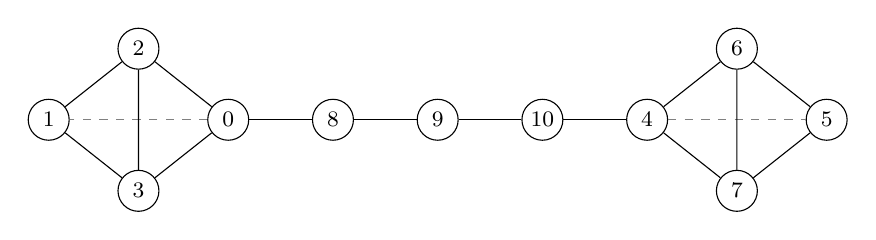
\begin{tikzpicture}[scale=0.95, every node/.style={circle, draw, fill=white, inner sep=0pt,
  minimum size=5.2mm, font=\footnotesize}]
\node (1) at (0,0) {1};
\node (2) at (1.2,0.95) {2};
\node (3) at (1.2,-0.95) {3};
\node (0) at (2.4,0) {0};
\node (8) at (3.8,0) {8};
\node (9) at (5.2,0) {9};
\node (10) at (6.6,0) {10};
\node (4) at (8.0,0) {4};
\node (6) at (9.2,0.95) {6};
\node (7) at (9.2,-0.95) {7};
\node (5) at (10.4,0) {5};
\draw[dashed, gray] (0)--(1);
\draw[dashed, gray] (4)--(5);
\draw (0)--(2) (0)--(3) (1)--(2) (1)--(3) (2)--(3);
\draw (4)--(6) (4)--(7) (5)--(6) (5)--(7) (6)--(7);
\draw (0)--(8)--(9)--(10)--(4);
\end{tikzpicture}
\caption{The graph $G_{11}$. With the two dashed edges added it becomes the barbell graph made
of two copies of $K_4$ and a path.}\label{fig:G11}
\end{figure}

\begin{proposition}\label{prop:G11mu}
$z\tr Lz\le\frac{37}{8}\,z\tr z$ for every $z\in\R^{11}$; hence $\mu_1(G_{11})\le\frac{37}{8}$.
\end{proposition}

\begin{proof}
For real numbers $a,b,c,e,p,q$ put
\begin{align*}
S(a,b,c,e,p,q)={}&\tfrac{8}{21}\bigl(\tfrac{21}{8}b+c+e\bigr)^2
+\tfrac{13}{14}\bigl(\tfrac{14}{13}a+c+e\bigr)^2
+\tfrac{13}{7}\bigl(\tfrac{7}{13}a+p\bigr)^2\\
&+\tfrac{17}{13}\bigl(\tfrac{13}{17}p+q\bigr)^2
+\tfrac{1}{336}(c+e)^2+\tfrac{5}{16}(c-e)^2\\
&+\tfrac{1}{104}a^2+\tfrac{3}{952}p^2 .
\end{align*}
Expanding both sides one checks the identity
\[
\tfrac{37}{8}\sum_{i=0}^{10}z_i^2-z\tr Lz
=S(z_0,z_1,z_2,z_3,z_8,z_9)+S(z_4,z_5,z_6,z_7,z_{10},z_9)+\tfrac{1}{104}z_9^2 ,
\]
whose right-hand side is a sum of $17$ squares with positive coefficients. The second assertion
follows from Lemma~\ref{lem:upper}.
\end{proof}

\begin{proposition}\label{prop:G11lambda}
$\lambda_2(G_{11})\ge\frac{293}{111}$.
\end{proposition}

\begin{proof}
Let $f=(7,6,8,8,0,0,0,0,3,0,0)$ and $g=(0,0,0,0,7,6,8,8,0,0,3)$. The support of $f$ is
$\{0,1,2,3,8\}$ and that of $g$ is $\{4,5,6,7,10\}$; they are disjoint and no edge joins them.
By \eqref{eq:forms},
\[
f\tr Af=2\,(7\cdot8+7\cdot8+6\cdot8+6\cdot8+8\cdot8+7\cdot3)=586,\qquad f\tr f=222,
\]
and the same holds for $g$. Since $586/222=293/111$, Lemma~\ref{lem:two} applies.
\end{proof}

\begin{proof}[Proof of Theorem~\ref{thm:G11}]
By the two propositions,
$\lambda_2-(\mu_1-2)\ge\frac{293}{111}-\frac{37}{8}+2=\frac{13}{888}$.
\end{proof}

\begin{remark}\label{rem:exact}
Deleting the vertex $9$ leaves two copies of a diamond with a pendant vertex, whose
characteristic polynomial is $(x+1)(x^4-x^3-5x^2+x+2)$. By Lemma~\ref{lem:interlace},
$\lambda_2(G_{11})$ is the largest root of $x^4-x^3-5x^2+x+2$, which is $2.64118\ldots$.
Numerically $\mu_1(G_{11})=4.61803\ldots$; the number $(7+\sqrt5)/2$ is a Laplacian eigenvalue of
$G_{11}$, and numerically it is the largest. So the true value of $\lambda_2-(\mu_1-2)$ is about
$0.0232$.
\end{remark}

\begin{remark}\label{rem:barbell}
The graph $G_{11}$ was found by a local search over non-bipartite graphs (bipartite graphs are
excluded by Proposition~\ref{prop:necessary}). It differs by two edges from the barbell graph
$B$ obtained from two copies of $K_4$ and the same path. In $B$ the two attachment vertices have
degree $4$, so $\mu_1(B)\ge5$ by Lemma~\ref{lem:degree}; numerically $\mu_1(B)=5.128$ and
$\lambda_2(B)=3.086$, a gap of $2.042$. In our computations with two copies of $K_m$ joined by
a path, $3\le m\le12$, the gap $\mu_1-\lambda_2$ decreases to $2$ from above as the path grows,
so barbells appear to support the conjecture. Removing one edge at each attachment vertex
lowers the maximum degree to $3$: then $\mu_1$ falls by $0.510$ and $\lambda_2$ by only $0.445$.
\end{remark}

\section{An infinite family}\label{sec:family}

For $k\ge3$ let $D_k$ be the graph obtained from two diamonds by joining a vertex of degree $2$
of the first to a vertex of degree $2$ of the second by a path with $k$ inner vertices
$p_1,\dots,p_k$. It has $k+8$ vertices, and $D_3=G_{11}$.

\begin{lemma}\label{lem:path}
Let $r\ge2$ and $y_0,\dots,y_r\in\R$. Then
\[
\sum_{i=0}^{r-1}(y_i-y_{i+1})^2\ \le\ \tfrac{30}{17}\,(y_0^2+y_r^2)+\tfrac{37}{8}\sum_{i=1}^{r-1}y_i^2 .
\]
\end{lemma}

\begin{proof}
For $t>0$ we have $(a-b)^2\le(1+t)a^2+(1+t^{-1})b^2$. With $t=\frac{13}{17}$ this reads
$(a-b)^2\le\frac{30}{17}a^2+\frac{30}{13}b^2$, and with $t=1$ it reads $(a-b)^2\le2a^2+2b^2$. Use
the first form for the first edge, with the weight $\frac{30}{17}$ on $y_0$, and for the last
edge, with the weight $\frac{30}{17}$ on $y_r$; use the second form for all other edges. An
inner vertex then receives at most
$\max\bigl(\frac{30}{13}+\frac{30}{13},\ \frac{30}{13}+2,\ 4\bigr)=\frac{60}{13}<\frac{37}{8}$.
\end{proof}

\begin{lemma}\label{lem:diamond}
For all real numbers $a,b,c,e,p$,
\begin{multline*}
(a-c)^2+(a-e)^2+(b-c)^2+(b-e)^2+(c-e)^2+(p-a)^2\\
\le\ \tfrac{37}{8}\,(a^2+b^2+c^2+e^2)+\tfrac{20}{7}\,p^2 .
\end{multline*}
\end{lemma}

\begin{proof}
The difference of the two sides equals
\[
\tfrac{8}{21}\bigl(\tfrac{21}{8}b+c+e\bigr)^2+\tfrac{13}{14}\bigl(\tfrac{14}{13}a+c+e\bigr)^2
+\tfrac{13}{7}\bigl(\tfrac{7}{13}a+p\bigr)^2+\tfrac{1}{336}(c+e)^2+\tfrac{5}{16}(c-e)^2+\tfrac{1}{104}a^2 .
\qedhere
\]
\end{proof}

The left-hand side of Lemma~\ref{lem:diamond} is the Laplacian form of a diamond on $a,b,c,e$
with missing edge $ab$, together with one further edge $pa$.

\begin{proposition}\label{prop:family}
For every $k\ge3$ we have $\mu_1(D_k)\le\frac{37}{8}$ and $\lambda_2(D_k)\ge\frac{293}{111}$.
\end{proposition}

\begin{proof}
Let $z$ be a vector indexed by the vertices of $D_k$. Split $z\tr Lz$ into three parts: the five
edges of the first diamond together with the edge to $p_1$; the same for the second diamond and
$p_k$; and the $k-1$ edges of the path $p_1,\dots,p_k$. Lemma~\ref{lem:diamond} bounds each of
the first two parts by $\frac{37}{8}$ times the squares on the diamond plus $\frac{20}{7}z_{p_1}^2$,
respectively $\frac{20}{7}z_{p_k}^2$. Lemma~\ref{lem:path} with $r=k-1\ge2$ bounds the third
part. The vertices $p_1$ and $p_k$ receive the weight
$\frac{20}{7}+\frac{30}{17}=\frac{550}{119}<\frac{37}{8}$, and every other vertex at most
$\frac{37}{8}$. Hence $z\tr Lz\le\frac{37}{8}z\tr z$, and Lemma~\ref{lem:upper} gives the first
claim.

For the second, take the vector with values $7,6,8,8$ on the first diamond ($7$ at the vertex
joined to $p_1$, $6$ at the other vertex of degree $2$), $3$ at $p_1$ and $0$ elsewhere, and its
mirror image on the second diamond and $p_k$. The computation in the proof of
Proposition~\ref{prop:G11lambda} applies verbatim; the two supports are joined by no edge
because $p_1$ and $p_k$ are distinct and not adjacent.
\end{proof}

\begin{proof}[Proof of Theorem~\ref{thm:family}]
Take $G=D_{n-8}$. By Proposition~\ref{prop:family}, the difference
$\lambda_2(G)-(\mu_1(G)-2)$ is at least $\frac{13}{888}$.
\end{proof}

\begin{remark}
Numerically $\mu_1(D_k)-\lambda_2(D_k)$ decreases from $1.9768$ at $k=3$ to $1.9226$ as
$k\to\infty$. Larger blocks do better: with $K_{d+1}$ minus an edge in place of the diamonds the
gap falls below $2$ already for shorter paths, and for large $d$ it appears to approach the
golden ratio $1.618\ldots$; compare Remark~\ref{rem:theta}.
\end{remark}

\section{The best constant}\label{sec:sharp}

\begin{definition}
Let $m\ge2$ and $s\ge2$. A \emph{cluster} $C(m,s)$ is the complete split graph with a clique
$K$ on $m$ vertices, the \emph{core}, and an independent set $W$ of $s$ vertices, the
\emph{satellites}, every satellite being joined to every core vertex. The graph $T(m,s)$
consists of two disjoint clusters $C(m,s)$ and a \emph{connector} vertex $c$ joined to one
satellite of each cluster; these two satellites are the \emph{attachment vertices}.
\end{definition}

The graph $T(m,s)$ has $2(m+s)+1$ vertices. Core vertices have degree $m+s-1$, attachment
vertices $m+1$, the other satellites $m$, and the connector $2$; so $\Delta=m+s-1$.

\begin{figure}[ht]
\centering
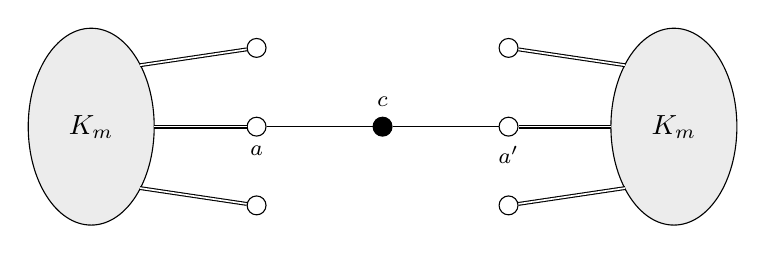
\begin{tikzpicture}[scale=1, dot/.style={circle, draw, fill=white, inner sep=0pt, minimum size=2.4mm}]
\draw[fill=gray!15] (0,0) ellipse (0.8 and 1.25);
\node at (0,0) {$K_m$};
\node[dot] (b1) at (2.1,1.0) {};
\node[dot, label=below:{\footnotesize $a$}] (a) at (2.1,0) {};
\node[dot] (b2) at (2.1,-1.0) {};
\draw[double] (b1) -- (0.62,0.78);
\draw[double] (a) -- (0.8,0);
\draw[double] (b2) -- (0.62,-0.78);
\node[dot, fill=black, label=above:{\footnotesize $c$}] (c) at (3.7,0) {};
\draw[fill=gray!15] (7.4,0) ellipse (0.8 and 1.25);
\node at (7.4,0) {$K_m$};
\node[dot] (d1) at (5.3,1.0) {};
\node[dot, label=below:{\footnotesize $a'$}] (ap) at (5.3,0) {};
\node[dot] (d2) at (5.3,-1.0) {};
\draw[double] (d1) -- (6.78,0.78);
\draw[double] (ap) -- (6.6,0);
\draw[double] (d2) -- (6.78,-0.78);
\draw (a) -- (c) -- (ap);
\end{tikzpicture}
\caption{The graph $T(m,s)$, drawn with $s=3$. A double line means that the satellite is joined
to every vertex of the clique.}\label{fig:T}
\end{figure}

\begin{lemma}[cluster inequality]\label{lem:cluster}
Let $C=C(m,s)$ with core $K$ and satellites $W$, let $a\in W$, and let $z\in\R^{K\cup W}$. Then
\[
\sum_{uv\in E(C)}(z_u-z_v)^2+2z_a^2\ \le\ \Bigl(m+s+\frac{3}{s}\Bigr)\sum_{v\in K\cup W}z_v^2 .
\]
\end{lemma}

\begin{proof}
Write $\sigma=\sum_{v\in K}z_v$, $P=\sum_{v\in K}z_v^2$, $\alpha=z_a$,
$\omega=\sum_{v\in W\setminus\{a\}}z_v$ and $Q=\sum_{v\in W\setminus\{a\}}z_v^2$. The edges inside
the core contribute $mP-\sigma^2$ and the edges between the core and the satellites contribute
$sP-2\sigma(\alpha+\omega)+m(\alpha^2+Q)$. With $\eta=3/s$, a direct computation gives
\begin{multline*}
(m+s+\eta)(P+\alpha^2+Q)-\bigl(mP-\sigma^2\bigr)-\bigl(sP-2\sigma(\alpha+\omega)+m(\alpha^2+Q)\bigr)-2\alpha^2\\
=\eta P+(\sigma+\alpha+\omega)^2+\bigl[(s+\eta-3)\alpha^2-2\alpha\omega+(s+\eta)Q-\omega^2\bigr].
\end{multline*}
By the Cauchy--Schwarz inequality $\omega^2\le(s-1)Q$, so the bracket is at least
\[
(s+\eta-3)\,\alpha^2-2\alpha\omega+\frac{1+\eta}{s-1}\,\omega^2 .
\]
This quadratic form in $(\alpha,\omega)$ is positive semidefinite: its coefficients
$s+\eta-3=s+\frac3s-3$ and $\frac{1+\eta}{s-1}$ are positive for $s\ge2$, and
\[
(s+\eta-3)(1+\eta)-(s-1)=\Bigl(1-\frac{3}{s}\Bigr)^2\ \ge\ 0 .\qedhere
\]
\end{proof}

\begin{proposition}\label{prop:Tmu}
$\mu_1\bigl(T(m,s)\bigr)\le m+s+\frac{3}{s}$.
\end{proposition}

\begin{proof}
Let $z$ be a vector on the vertices of $T(m,s)$ and let $a,a'$ be the attachment vertices. For
the two edges at the connector, $(z_c-z_a)^2\le2z_c^2+2z_a^2$ and likewise for $a'$. Therefore
$z\tr Lz$ is at most $4z_c^2$ plus, for each cluster, its Laplacian form plus twice the square at
its attachment vertex. By Lemma~\ref{lem:cluster}, and since $4\le m+s+\frac3s$, we get
$z\tr Lz\le(m+s+\frac3s)\,z\tr z$. Conclude with Lemma~\ref{lem:upper}.
\end{proof}

\begin{proposition}\label{prop:Tlambda}
$\lambda_2\bigl(T(m,s)\bigr)\ge\dfrac{m(m-1)+2ms}{m+s}$.
\end{proposition}

\begin{proof}
Let $f$ and $g$ be the indicator vectors of the two clusters. Their supports are disjoint and
joined by no edge, because the connector belongs to neither. A cluster has
$\binom m2+ms$ edges, so $f\tr Af=m(m-1)+2ms$ by \eqref{eq:forms}, and $f\tr f=m+s$; the same
holds for $g$. Apply Lemma~\ref{lem:two}.
\end{proof}

Subtracting, and using $(m+s)^2-m(m-1)-2ms=m+s^2$, we obtain \eqref{eq:gapbound}:

\begin{theorem}\label{thm:gap}
For all $m\ge2$ and $s\ge2$,
\[
\mu_1\bigl(T(m,s)\bigr)-\lambda_2\bigl(T(m,s)\bigr)\ \le\ 1+\frac{3}{s}+\frac{s^2-s}{m+s} .
\]
\end{theorem}

\begin{proof}[Proof of Theorem~\ref{thm:sharp}]
If $c\le1$ the inequality holds by \eqref{eq:known}. Let $c>1$ and choose an integer $s\ge2$
with $4/s<c-1$. For $m=s^3$ we have $\frac{s^2-s}{m+s}<\frac1s$, so Theorem~\ref{thm:gap} gives
$\mu_1-\lambda_2<1+\frac4s<c$ for the connected graph $T(s^3,s)$.
\end{proof}

The lower bound of Proposition~\ref{prop:Tlambda} is the average degree of a cluster. The exact
value is also available.

\begin{proposition}\label{prop:exact}
$\lambda_2\bigl(T(m,s)\bigr)=\dfrac{(m-1)+\sqrt{(m-1)^2+4ms}}{2}$, the largest adjacency
eigenvalue of $C(m,s)$.
\end{proposition}

\begin{proof}
Deleting the connector leaves two copies of $C(m,s)$, so Lemma~\ref{lem:interlace} applies. The
Perron vector of $C(m,s)$ is constant on the core and on the satellites, and
$\lambda_1(C(m,s))$ is the largest eigenvalue of the quotient matrix
$\bigl(\begin{smallmatrix}m-1&s\\ m&0\end{smallmatrix}\bigr)$, that is, the largest root of
$x^2-(m-1)x-ms$.
\end{proof}

\begin{remark}\label{rem:theta}
For fixed $s$ and $m\to\infty$, numerical computation indicates that
\[
\mu_1\bigl(T(m,s)\bigr)-\lambda_2\bigl(T(m,s)\bigr)\ \longrightarrow\ \theta_s
=1+\frac{\sqrt{(s-1)^2+4}-(s-1)}{2},
\]
so that $\theta_2$ is the golden ratio, $\theta_3=\sqrt2$, and $\theta_s\to1$. We have not
proved this. The graph $T(m,2)$ is two copies of $K_{m+2}$ minus an edge joined by a path with
one inner vertex, which links this family to that of Section~\ref{sec:family}.
\end{remark}

\begin{corollary}\label{cor:linear}
Let $a,b\in\R$ be such that $\lambda_2(G)\le a\,\mu_1(G)+b$ for every connected graph $G$ with at
least two vertices. Then $a\ge1$, and if $a=1$ then $b\ge-1$.
\end{corollary}

\begin{proof}
Along the graphs $T(s^3,s)$ we have $\mu_1\ge\Delta+1\to\infty$ and $\mu_1-\lambda_2\to1$. If
$a<1$ then $a\mu_1+b-\lambda_2=(a-1)\mu_1+b+(\mu_1-\lambda_2)\to-\infty$, and if $a=1$ the same
quantity tends to $b+1$.
\end{proof}

\begin{corollary}
The inequality $\mu_2\ge\lambda_2+1$ of \cite[Theorem~1]{Cazenave} is asymptotically tight for
graphs with arbitrarily large $\lambda_2$: for every $\varepsilon>0$ and every $K$ there is a
connected graph with $\lambda_2>K$ and $\mu_2-\lambda_2<1+\varepsilon$.
\end{corollary}

\begin{proof}
$\mu_2\le\mu_1$, and $\lambda_2(T(s^3,s))\to\infty$ by Proposition~\ref{prop:Tlambda}.
\end{proof}

In \cite{Cazenave} equality in $\mu_2\ge\lambda_2+1$ is noted for stars, where $\lambda_2=0$.

\section{Where a counterexample can live}\label{sec:necessary}

\begin{proposition}\label{prop:necessary}
Let $G$ be a connected graph on $n\ge2$ vertices with $\lambda_2>\mu_1-2$. Then
\begin{enumerate}
\item[(i)] $G$ is not bipartite;
\item[(ii)] $\lambda_2>\Delta-1$;
\item[(iii)] $n\ge2\Delta+2$.
\end{enumerate}
In particular $\Delta\ge3$ and $n\ge8$.
\end{proposition}

\begin{proof}
(ii) is immediate from Lemma~\ref{lem:degree}(b).

(iii) Let $y$ be an eigenvector of $A$ for $\lambda_2$. It is orthogonal to the positive Perron
vector, so the sets $P=\{v:y_v>0\}$ and $N=\{v:y_v<0\}$ are both non-empty. For $v\in P$,
$\lambda_2y_v=\sum_{u\sim v}y_u\le\sum_{u\sim v,\,u\in P}y_u$. Multiplying by $y_v$ and summing
over $P$ gives $\lambda_2\sum_Py_v^2\le y_P\tr A[P]\,y_P$, so $\lambda_1(G[P])\ge\lambda_2$, and
similarly for $N$. A graph on $|P|$ vertices has largest eigenvalue at most $|P|-1$, hence
$|P|-1\ge\lambda_2>\Delta-1$ by (ii). So $|P|\ge\Delta+1$, likewise $|N|\ge\Delta+1$, and the two
sets are disjoint.

(i) Let $G$ be bipartite. Then $L$ is similar to $Q=D+A$ by a diagonal matrix of signs, so
$\mu_1$ is the largest eigenvalue of $Q$. If $x$ is the unit Perron vector of $A$, the proof of
Lemma~\ref{lem:degree}(a) shows $x\tr Dx\ge x\tr Ax=\lambda_1$, hence
$\mu_1\ge x\tr Qx\ge2\lambda_1$. If $\lambda_1\ge2$ this gives
$\mu_1\ge\lambda_1+2>\lambda_2+2$. If $\lambda_1<2$ then, by a theorem of Smith
\cite{Smith} (see \cite[Section~3.1]{BrouwerHaemers}), $G$ is a path or one of the trees
$D_n$, $E_6$, $E_7$, $E_8$. The latter have $\Delta=3$, so $\mu_1\ge4>\lambda_2+2$. For the path
on $n$ vertices, $\mu_1-2=2\cos\frac{\pi}{n}>2\cos\frac{2\pi}{n+1}=\lambda_2$.

Finally, if $\Delta\le2$ then $G$ is a path or a cycle; paths are bipartite, and for the cycle
$C_n$ one has $\mu_1\ge4-4\sin^2\frac{\pi}{2n}$ and $\lambda_2=2\cos\frac{2\pi}{n}$, so
$\mu_1-\lambda_2\ge2$. Hence $\Delta\ge3$, and $n\ge8$ by (iii).
\end{proof}

Since all connected graphs with at most $9$ vertices satisfy the conjecture \cite{Cazenave},
the smallest counterexample has $10$ or $11$ vertices.

\section{The Randi\'c index and the rest of the corpus}\label{sec:randic}

\subsection{Cluster graphs with two satellites}

\begin{proof}[Proof of Theorem~\ref{thm:randic}]
Let $a$ be an attachment vertex, $b$ the other satellite of its cluster, and use primes for the
second cluster. From the connector $c$ the distances are $1$ to $a$, $2$ to the core and $3$ to
$b$, so $c$ has eccentricity $3$. The eccentricities of $a$, of a core vertex and of $b$ are
$4$, $5$ and $6$, attained at $b'$ in each case. Hence the radius is $3$ and the diameter $6$.

The degrees are $m+1$ on the core and at $a$, $m$ at $b$ and $2$ at $c$. One cluster with its
connector edge contributes to $R$
\begin{multline*}
\binom m2\frac{1}{m+1}+\frac{m}{m+1}+\frac{m}{\sqrt{m(m+1)}}+\frac{1}{\sqrt{2(m+1)}}\\
=\frac m2+\sqrt{\frac{m}{m+1}}+\frac{1}{\sqrt{2(m+1)}} ,
\end{multline*}
which gives the formula for $R$. The formula for $\lambda_2$ is Proposition~\ref{prop:exact}
with $s=2$. Finally $\sqrt{m^2+6m+1}=m+3+o(1)$, so $\lambda_2=m+1+o(1)$ and $R=m+2+o(1)$.
\end{proof}

\begin{corollary}\label{cor:rows}
Each of the inequalities in Table~\ref{tab:rows} fails on $T(m,2)$ for all sufficiently large
$m$.
\end{corollary}

\begin{proof}
On $T(m,2)$ every inequality of the first ten lines reads $\lambda_2\le R-c$ with the constant
$c>1$ of the third column, and $R-\lambda_2\to1$. For the last line, the maximum is attained at a
vertex of maximum degree $m+1$, and $n=2m+5$; so the right-hand side is
$R\sqrt{(m+1)/(m+4)}=m+\frac12+o(1)$, while $\lambda_2=m+1+o(1)$.
\end{proof}

\begin{table}[ht]
\centering
\footnotesize
\begin{tabular}{@{}lllr@{}}
\toprule
corpus numbers & inequality & $c$ on $T(m,2)$ & least $m$\\
\midrule
1053490, 861166 & $\lambda_2\le R-\rad/2$ & $1.5$ & $10$\\
2619484, 2619875, 2632018, & $\lambda_2\le R+1-\sqrt{\diam}$ & $\sqrt6-1\approx1.449$ & $12$\\
\quad 2632484, 2638219 & & &\\
2632674 & $\lambda_2\le R-\sqrt{\rad-1}$ & $\sqrt2\approx1.414$ & $15$\\
2632694 & $\lambda_2\le R-\sqrt{\rad/2}$ & $\sqrt{3/2}\approx1.225$ & $47$\\
2632494 & $\lambda_2\le R-\sqrt{\diam}/2$ & $\sqrt6/2\approx1.225$ & $47$\\
2632479 & $\lambda_2\le R-(\log\rad)^2$ & $(\log3)^2\approx1.207$ & $55$\\
806941, 2632538 & $\lambda_2\le R-\log\rad$ & $\log3\approx1.099$ & $225$\\
2632658, 2632739 & $\lambda_2\le R-\log(\diam/2)$ & $\log3\approx1.099$ & $225$\\
1053530 & $\lambda_2\le R-\sqrt{\log\rad}$ & $\approx1.048$ & $903$\\
2632774 & $\lambda_2\le R-\sqrt[4]{\log\rad}$ & $\approx1.024$ & $3617$\\
\midrule
708247 & $\lambda_2\le\max_v R\sqrt{d_v/(n-d_v)}$ & & $14$\\
\bottomrule
\end{tabular}
\smallskip
\caption{Open conjectures of the corpus of \cite{Cazenave,DuhamelCazenave} refuted by the
graphs $T(m,2)$. Numbers on one line are rewritings of the same inequality. The last column is
the least $m$ for which $T(m,2)$ violates the inequality, obtained by evaluating the formulas of
Theorem~\ref{thm:randic}; $T(m,2)$ has $2m+5$ vertices. Logarithms are natural.}\label{tab:rows}
\end{table}

\subsection{A counterexample on ten vertices}
Smaller counterexamples to some of these inequalities exist among the graphs of
Section~\ref{sec:family} with larger blocks and shorter paths. We give one in full.

\begin{proposition}\label{prop:H10}
Let $H_{10}$ be the graph obtained from two copies of $K_5$ by deleting one edge $uw$ in the
first and one edge $u'w'$ in the second and adding the edge $uu'$. Then $\rad(H_{10})=3$ and
$R(H_{10})=\frac{13}{4}+\sqrt3$, so that $R(H_{10})-\frac12\rad(H_{10})=\frac74+\sqrt3$, and
\[
\lambda_2(H_{10})\ \ge\ \frac{146244}{41581}\ >\ \frac74+\sqrt3 .
\]
\end{proposition}

\begin{proof}
The vertices $u,u'$ have eccentricity $3$, attained at $w'$ and $w$, and every other vertex has
larger eccentricity. The vertices $w,w'$ have degree $3$ and all other vertices degree $4$, so
$R=2\bigl(\frac34+\frac{3}{\sqrt{12}}+\frac34\bigr)+\frac14=\frac{13}{4}+\sqrt3$.

Let $x$ be the vector on the first copy with $x_u=66$, $x_w=85$ and value $100$ on the three
remaining vertices, let $x'$ be its copy on the second, and put $f=(x,x')$ and $g=(x,-x')$.
Then $f\tr g=0$. Each copy contributes $2(66\cdot300+85\cdot300+3\cdot100^2)=150600$ to the
quadratic form of $A$, and the edge $uu'$ contributes $\pm2\cdot66^2$. So
\[
g\tr Ag=2\cdot150600-2\cdot66^2=292488,\qquad f\tr f=g\tr g=83162,
\]
while $f\tr Af\ge g\tr Ag$ and $f\tr Ag=150600-150600+66^2-66^2=0$. Lemma~\ref{lem:two} gives
$\lambda_2\ge292488/83162=146244/41581$. Finally
\[
\Bigl(\frac{146244}{41581}-\frac74\Bigr)^2=\frac{86382500281}{27663672976}>3 .\qedhere
\]
\end{proof}

Thus the corpus conjecture $\lambda_2\le R-\rad/2$ (number 1053490) already fails on $10$
vertices, the first order not covered by the exhaustive test of \cite{Cazenave}. Numerically
$\lambda_2(H_{10})=3.5171$ and $R-\rad/2=3.4821$.

\subsection{Numerical evidence on the whole corpus}
We evaluated every conjecture marked open in the archive of \cite{Cazenave}, $14{,}150$ in all,
on the graphs of Sections~\ref{sec:family} and~\ref{sec:sharp} and their variants: $936$ graphs
with at most $1041$ vertices, and $193$ graphs $T(m,s)$ with up to two million vertices, whose
invariants were computed from the quotient by their classes of twin vertices. A conjecture was
counted as violated when the left-hand side exceeded the right-hand side by more than
$10^{-6}$, the threshold used in the corpus, in floating-point arithmetic, and when this
persisted under perturbations of the eigenvalues and of $R$ of relative size $10^{-9}$.

In this sense $125$ of the open conjectures are violated. They include the four with left-hand
side $\lambda_2$ and right-hand side $\mu_1-c$ (Theorem~\ref{thm:sharp}) and the eighteen of
Table~\ref{tab:rows}. For the remaining $103$ the special structure of our graphs plays no
role: each is also violated by two complete graphs joined by an edge, on $62$ vertices or more.
The test graphs of the corpus include that family up to $60$ vertices. None of the $117{,}390$
conjectures marked as proved in the archive was violated on any of our graphs, and our
evaluator reproduces the margin recorded in the archive for $61{,}074$ of the $61{,}115$ refuted
conjectures whose recorded counterexample has at most $6$ vertices; the $41$ exceptions are
expressions evaluated at a singular point. The list of violated conjectures and the program
are in the repository named in Section~\ref{sec:lean}. Apart from the statements proved above,
these are numerical observations and not theorems.

Conjecture~1 of \cite{Cazenave}, $R\ge\lambda_2+1$, held on all these graphs, as did the other
five conjectures highlighted there.

\section{Formalization}\label{sec:lean}

The statements listed in Table~\ref{tab:lean} are formalized in Lean~4 \cite{Lean4} with
Mathlib \cite{Mathlib}, both at version \texttt{v4.36.0-rc1}. The development has nine files
and about $1950$ lines. It is available at
\url{https://github.com/Sulayman22S/gap-is-one}, together with the programs and the data of
Section~\ref{sec:randic}. The two eigenvalue tests are derived from the spectral theorem of
Mathlib.

\begin{table}[ht]
\centering
\footnotesize
\begin{tabular}{@{}ll@{}}
\toprule
statement & name in the development\\
\midrule
Lemma~\ref{lem:upper} & \lean{eigenvalues\textsubscript{0}\_le\_of\_quadForm\_le}\\
Lemma~\ref{lem:two} & \lean{le\_eigenvalues\textsubscript{0}\_one}\\
Lemma~\ref{lem:degree}(a) & \lean{adj\_quadForm\_le}\\
Lemma~\ref{lem:degree}(b) & \lean{maxDegree\_add\_one\_le\_mu\textsubscript{1}}\\
the bound \eqref{eq:known} & \lean{lambda\textsubscript{2}\_le\_mu\textsubscript{1}\_sub\_one}\\
Proposition~\ref{prop:G11mu} & \lean{mu\textsubscript{1}\_G11\_le}\\
Proposition~\ref{prop:G11lambda} & \lean{lambda\textsubscript{2}\_G11\_ge}\\
Theorem~\ref{thm:G11} & \lean{counterexample\_gap}, \lean{conjecture\_two\_false}\\
Lemma~\ref{lem:path} & \lean{path\_both}\\
Lemma~\ref{lem:diamond} & \lean{diamond\_attach\_le}\\
Proposition~\ref{prop:family} & \lean{mu\textsubscript{1}\_fam\_le}, \lean{lambda\textsubscript{2}\_fam\_ge}\\
Theorem~\ref{thm:family} & \lean{family\_gap}, \lean{exists\_counterexample}\\
Lemma~\ref{lem:cluster} & \lean{cluster\_le}\\
Theorem~\ref{thm:gap} and its two propositions & \lean{exists\_gap\_le}\\
Theorem~\ref{thm:sharp} & \lean{best\_constant}\\
the case $c=\sqrt2$ & \lean{conjecture\_sqrt\_two\_false}\\
the case $c=\sqrt[4]{2}$ & \lean{conjecture\_fourth\_root\_two\_false}\\
\bottomrule
\end{tabular}
\smallskip
\caption{Formalized statements and their names in the Lean development.}\label{tab:lean}
\end{table}

The main statement reads
\begin{multline*}
\forall c\in\R,\quad\Bigl(\forall n\ge2,\ \forall G:\texttt{SimpleGraph (Fin }n\texttt{)},\\
G\ \text{connected}\ \Rightarrow\ \lambda_2(G)\le\mu_1(G)-c\Bigr)\ \Longleftrightarrow\ c\le1 .
\end{multline*}
Here $\lambda_2(G)$ and $\mu_1(G)$ are the entries of index $1$ and $0$ of the decreasing list
of eigenvalues, with multiplicity, of the adjacency and the Laplacian matrix of $G$ over $\R$;
Mathlib calls this list \lean{eigenvalues\textsubscript{0}}. These are also the conventions of
the Lean library that accompanies \cite{Cazenave}. The graphs $T(m,s)$ are defined on a
structured vertex type, and the bounds are transferred to \texttt{Fin}~$n$ along a bijection.

The proofs depend only on the three standard axioms of Lean with Mathlib
(\lean{propext}, \lean{Classical.choice}, \lean{Quot.sound}) and contain no \lean{sorry}. As a
check against vacuity, twelve false variants of the statements, such as the claim that the
constant $1$ also fails, were confirmed to be rejected. Three headline
statements, namely that Conjecture~2 is false, Theorem~\ref{thm:family} and
Theorem~\ref{thm:sharp}, are also given on their own in a file \texttt{Challenge.lean} that
imports only Mathlib. The tool \texttt{lake comparator} confirms that the development proves
exactly these statements, and it replays the proofs through two further proof checkers.

Not formalized: the strict inequality $\lambda_2<\mu_1-1$, Lemma~\ref{lem:interlace},
Proposition~\ref{prop:exact}, the corollaries of Section~\ref{sec:sharp},
Proposition~\ref{prop:necessary}, and all of Section~\ref{sec:randic}. In the formal proof of
Theorem~\ref{thm:sharp} the parameters are $s>4/(c-1)$ and $m=s^3$, as above.

Two of the formalized lemmas may be of independent use. The lemma table of the Lean library of
\cite{Cazenave} lists $2m/n\le\lambda_1\le\Delta$ and
$\Delta+1\le\mu_1\le\min(n,2\Delta)$ among the lemmas that are used by its proof search but not
yet formalized; one half of each is Lemma~\ref{lem:degree}.

\section{Questions}\label{sec:questions}

\begin{question}
Is there a connected graph on $10$ vertices with $\lambda_2>\mu_1-2$? By
Proposition~\ref{prop:necessary} such a graph is not bipartite and has maximum degree $3$ or
$4$.
\end{question}

\begin{question}
For $\Delta\ge2$ let $g(\Delta)$ be the infimum of $\mu_1-\lambda_2$ over connected graphs with
maximum degree $\Delta$. Then $g(2)=2$, and $g(\Delta)\to1$ by Theorem~\ref{thm:gap}. Determine
$g(3)$. The graphs $D_k$ give $g(3)\le2-\frac{13}{888}$, and numerically $g(3)\le1.9226$.
\end{question}

\begin{question}
Prove the limit formula of Remark~\ref{rem:theta}.
\end{question}

\begin{question}
Is $R\ge\lambda_2+1$ for every connected graph \cite[Conjecture~1]{Cazenave}? By
Theorem~\ref{thm:randic} no term depending on the radius or the diameter can be added to the
right-hand side.
\end{question}

\subsection*{How this work was made}
The first counterexample was found by a computer search. The constructions, the proofs, the
Lean formalization, the programs and the text of this paper were produced by an AI system
(Claude, Anthropic, used through Claude Code), working under the direction of the author. All
formal proofs were checked by the Lean kernel; Section~\ref{sec:lean} lists the statements that
are proved only by hand.

\begin{thebibliography}{99}

\bibitem{BrouwerHaemers}
A. E. Brouwer and W. H. Haemers, \emph{Spectra of Graphs}, Universitext, Springer, New York,
2012.

\bibitem{CaporossiHansen}
G. Caporossi and P. Hansen, Variable neighborhood search for extremal graphs. 1. The
AutoGraphiX system, \emph{Discrete Math.} \textbf{212} (2000), 29--44.

\bibitem{Cazenave}
T. Cazenave, Lemmas and conjectures in spectral graph theory, preprint, arXiv:2611.03879,
2026.

\bibitem{DuhamelCazenave}
E. Duhamel and T. Cazenave, Spectral graph theory conjecture generation, AAAI 2026 Workshop
\emph{AI for Research}, 2026.

\bibitem{Fajtlowicz}
S. Fajtlowicz, On conjectures of Graffiti, \emph{Discrete Math.} \textbf{72} (1988), 113--118.

\bibitem{GroneMerris}
R. Grone and R. Merris, The Laplacian spectrum of a graph. II, \emph{SIAM J. Discrete Math.}
\textbf{7} (1994), 221--229.

\bibitem{HornJohnson}
R. A. Horn and C. R. Johnson, \emph{Matrix Analysis}, 2nd ed., Cambridge University Press,
Cambridge, 2013.

\bibitem{LinHongShu}
H. Lin, Y. Hong and J. Shu, Some relations between the eigenvalues of adjacency, Laplacian and
signless Laplacian matrix of a graph, \emph{Graphs Combin.} \textbf{31} (2015), 669--677.

\bibitem{Mathlib}
The mathlib Community, The Lean mathematical library, in \emph{Proceedings of the 9th ACM SIGPLAN
International Conference on Certified Programs and Proofs (CPP 2020)}, ACM, 2020, pp. 367--381.

\bibitem{Lean4}
L. de Moura and S. Ullrich, The Lean 4 theorem prover and programming language, in
\emph{Automated Deduction -- CADE 28}, Lecture Notes in Comput. Sci. 12699, Springer, 2021,
pp. 625--635.

\bibitem{Randic}
M. Randi\'c, On characterization of molecular branching, \emph{J. Amer. Chem. Soc.} \textbf{97}
(1975), 6609--6615.

\bibitem{Smith}
J. H. Smith, Some properties of the spectrum of a graph, in \emph{Combinatorial Structures and
their Applications}, Gordon and Breach, New York, 1970, pp. 403--406.

\bibitem{Zhang}
X.-D. Zhang, The Laplacian eigenvalues of graphs: a survey, preprint, arXiv:1111.2897, 2011.

\end{thebibliography}

\end{document}
